





% Adjust row height
\renewcommand{\arraystretch}{0.1} % Reduce row height




%====================================================================
%                      PACKAGES


%====================================================================
%                      DOCUMENT
%====================================================================


%------------------------------------------------------------------
% فصل (یا Chapter) اول
%------------------------------------------------------------------
\chapter{روش‌ها}

%------------------------------------------------------------------
%                           SECTION 1
%------------------------------------------------------------------
\section{مقدمه}
پیش‌پردازش داده‌ها یکی از مراحل اصلی در فرآیند تحلیل و آماده‌سازی داده‌ها است که به منظور بهبود کیفیت داده‌ها و فراهم کردن اطلاعات مناسب برای استفاده در مدل‌سازی و تحلیل انجام می‌شود. داده‌های خام معمولاً شامل اطلاعات ناقص، نویز یا ویژگی‌های نامتناسب هستند که می‌توانند بر کیفیت تحلیل و نتایج تأثیر منفی بگذارند. در این فصل، مراحل پیش‌پردازش داده‌های مربوط به پروژه شناسایی علائم راهنمایی و رانندگی توضیح داده خواهد شد.

%------------------------------------------------------------------
%                           SECTION 2
%------------------------------------------------------------------
\section{تغییر اندازه و نرمال‌سازی تصاویر}
در پیش‌پردازش داده‌ها، تغییر اندازه و نرمال‌سازی تصاویر دو مرحله اساسی برای هماهنگی و بهینه‌سازی داده‌های ورودی هستند. تصاویر خام در دیتاست اغلب ابعاد و مقیاس‌های متفاوتی دارند که می‌تواند پردازش آن‌ها را دشوار کرده و منجر به نتایج غیر دقیق شود. برای حل این مسئله، ابتدا تصاویر به ابعاد ثابت \(( N \times N )\) تغییر اندازه داده می‌شوند و سپس مقادیر پیکسل‌ها نرمال‌سازی می‌شوند تا مدل بتواند به طور بهینه‌تری یادگیری را انجام دهد.

فرآیند تغییر اندازه تصاویر به این صورت است که تمامی تصاویر ورودی به ابعاد ثابت \(( N \times N )\) بازنمونه‌گیری می‌شوند. این بازنمونه‌گیری با استفاده از روش‌هایی مانند بایلاینر\footnote{Bilinear} یا نزدیک‌ترین همسایه\footnote{Nearest Neighbor} انجام می‌شود. فرمول ریاضی تغییر اندازه برای نگاشت تصویر \( I \) با ابعاد اولیه \(( H \times W )\) به تصویر \( I' \) با ابعاد \(( N \times N )\) به صورت زیر است:
\[
I'(x', y') = I\Bigl( x \cdot \frac{H}{N}, \; y \cdot \frac{W}{N}\Bigr)
\]
که در آن:
\begin{itemize}
    \item \( I'(x',y') \): مقدار پیکسل در تصویر تغییر اندازه داده‌شده
    \item \( I(x,y) \): مقدار پیکسل در تصویر اصلی
    \item \( H, W \): ارتفاع و عرض تصویر اولیه
    \item \( N \): ابعاد جدید تصویر
\end{itemize}

در مرحله نرمال‌سازی، مقادیر پیکسل‌ها که معمولاً در بازه \([0, 255]\) قرار دارند، به بازه \([0, 1]\) نگاشت می‌شوند:
\[
p' = \frac{p}{255}
\]
که در آن:
\begin{itemize}
    \item \( p \): مقدار اصلی پیکسل
    \item \( p' \): مقدار نرمال‌شده پیکسل
\end{itemize}

برگشت‌پذیری نرمال‌سازی نیز با معادله زیر انجام می‌شود:
\[
I_{\text{original}} = (I_{\text{normalized}} \times \sigma) + \mu
\]
کاربردهای برگشت‌پذیری شامل نمایش یا ذخیره تصاویر به شکل اولیه و انجام تحلیل‌های اضافی بر تصاویر اصلی است.

برای هر تصویر \( I_{\text{original}} \) که شامل سه کانال رنگی (قرمز، سبز، آبی) است، نرمال‌سازی به صورت زیر انجام می‌شود:
\[
I_{\text{normalized}} = \frac{I_{\text{original}} - \mu}{\sigma}
\]
که در آن:
\begin{itemize}
    \item \( I_{\text{normalized}} \): مقدار پیکسل در تصویر نرمال‌شده
    \item \( I_{\text{original}} \): مقدار اصلی پیکسل در تصویر
    \item \(\mu\): میانگین مقادیر پیکسل برای هر کانال رنگی
    \item \(\sigma\): انحراف معیار مقادیر پیکسل برای هر کانال رنگی
\end{itemize}

این نرمال‌سازی باعث کاهش تأثیر ویژگی‌های با مقیاس بزرگ‌تر شده و همگرایی مدل را تسریع می‌کند. ترکیب این دو مرحله (تغییر اندازه و نرمال‌سازی) به مدل کمک می‌کند تا داده‌های ورودی را به شکلی استاندارد و بهینه پردازش کند.

\clearpage

%------------------------------------------------------------------
%                           SECTION 3
%------------------------------------------------------------------
%------------------------------------------------------------------
\section{بهبود بینایی ماشین با ادغام درک معنایی، استدلال شناختی و روان‌فیزیک}
سیستم‌های بینایی ماشین در دهه‌های اخیر با تحولات شگرفی روبه‌رو شده‌اند؛ به‌نحوی‌که از روش‌های ساده شناسایی اشیاء و تشخیص الگو فراتر رفته و به الگوریتم‌هایی دست یافته‌اند که قادرند مفاهیم پیچیده‌تری را درک کرده و دربارهٔ آن‌ها استدلال نمایند. بااین‌حال، در محیط‌های واقعی که پویا، ناهمگن و غیرقابل‌پیش‌بینی هستند، مدل‌های سنتی مبتنی بر استخراج ویژگی‌های خام یا الگوهای صرفاً آماری، با محدودیت مواجه می‌شوند. ترکیب درک معنایی، استدلال شناختی و روان‌فیزیک در یک چارچوب واحد، امکان ساخت سیستم‌های هوشمند و مقاوم‌تری را فراهم می‌سازد که نه‌تنها قادر به شناسایی اشیاء هستند، بلکه معنای آن‌ها را در بستر کاربردی و انسانی درک کرده، روابطشان را تحلیل نموده و واکنش‌های مناسبی از خود نشان می‌دهند. این رویکرد جامع همچنین توانایی سیستم‌های بینایی را در تعمیم دانش به موقعیت‌های جدید و تصمیم‌گیری در شرایط بحرانی یا ناآشنا بهبود می‌بخشد.

\section*{درک معنایی: از طبقه‌بندی ساده به تحلیل زمینه‌ای عمیق}
درک معنایی، توانایی سیستم برای فرا رفتن از سطح پیکسل‌ها و ویژگی‌های محاسباتی اولیه، و ورود به حوزهٔ معناداری اشیاء و صحنه است. برخلاف رویکردهای سنتی که تمرکزشان بر شناسایی برچسب اشیاء در سطحی ایستا بود، درک معنایی سعی می‌کند ساختار و بافت صحنه، همچنین عملکرد و جایگاه اشیاء را در محیط بررسی کند. این موضوع به‌ویژه در سامانه‌های خودران، رباتیک پیشرفته، و حوزه‌هایی مانند نظارت تصویری اهمیت می‌یابد، زیرا تعامل میان اشیاء، اهداف، و رفتارها می‌تواند تأثیر عمیقی بر نتیجهٔ نهایی داشته باشد. برای نمونه، تشخیص یک عابر پیاده در کنار خیابان به‌تنهایی کافی نیست؛ سیستم باید بفهمد که عابر احتمالاً قصد عبور دارد و به‌دلیل نزدیک بودن به خط عابر، باید سرعت خودرو کاهش یابد یا دستورات هشدار فعال شوند.

\subsection*{تولید گراف صحنه}
تولید گراف صحنه، یکی از روش‌های کلیدی در رسیدن به درک معنایی عمیق است. در این گراف، هر شیء به‌عنوان یک گره نمایش داده می‌شود و کنش‌ها یا روابط میان اشیاء مختلف از طریق یال‌ها مشخص می‌شوند. برای نمونه، در یک صحنهٔ شهری می‌توان شیئی به نام «خودرو» را شناسایی کرد و رابطهٔ «در حال حرکت به سمت» را میان آن و «تابلوی ایست» قرار داد. علاوه بر این، یک «عابر پیاده» نیز می‌تواند در رابطهٔ «نزدیک» با همین تابلو قرار گرفته باشد. این مدل‌سازی ساختارمند به سامانه اجازه می‌دهد فراتر از حضور صرف اشیاء رفته و تصمیمات یا پیش‌بینی‌های خود را بر پایهٔ روابط و بافت عمومی صحنه بنا کند.

\subsection*{هستان‌شناسی‌های سلسله‌مراتبی}
به‌جای آنکه هر شیء در طبقه‌بندی‌های مجزا و بدون ارتباط با یکدیگر تعریف شود، هستان‌شناسی‌های سلسله‌مراتبی تلاش دارند ساختاری لایه‌لایه از مفاهیم را ارائه دهند. به این ترتیب، اشیاء در رده‌بندی‌هایی از کلان به خرد تقسیم‌بندی می‌شوند و ویژگی‌های مشترک در سطوح بالاتر به اشتراک گذاشته می‌شود. برای مثال، مفهوم «خودرو» می‌تواند زیرمجموعه‌ای از «وسیله نقلیه» باشد که خود در سطح بالاتری به «وسیله حمل‌ونقل» متصل است. چنین رویکردی کمک می‌کند سیستم در صورت مواجهه با اشیاء جدید یا دسته‌بندی‌های ناشناخته، از روابط سلسله‌مراتبی برای تشخیص سریع‌تر و درک عمیق‌تر استفاده کند. این شیوه همچنین زمانی که داده‌های آموزشی محدود هستند، کارآمدتر خواهد بود؛ زیرا دانش به‌دست‌آمده از اشیاء یک رده می‌تواند برای شناسایی ردهٔ دیگری به‌کار گرفته شود.

\subsection*{مدل‌های ترکیب تصویر و زبان}
در کنار روش‌های مبتنی بر گراف و هستان‌شناسی، مدل‌هایی که از ترکیب اطلاعات زبانی و تصویری بهره می‌برند نیز نقش بسزایی در افزایش درک معنایی ایفا کرده‌اند. این مدل‌ها تلاش می‌کنند بین متن و تصویر ارتباط برقرار نمایند و به‌این‌ترتیب، اشیاء یا صحنه‌ها را نه‌فقط به‌صورت بصری، بلکه در چارچوب توصیف‌های زبانی هم تحلیل کنند. چنین رویکردی برای کاربردهایی مانند جستجوی تصویری متنی، زیرنویس‌گذاری خودکار تصاویر و ویدئوها، و حتی پاسخگویی به پرسش‌های متنی بر پایهٔ تصاویر بسیار سودمند است. هم‌افزایی دانش زبانی با ویژگی‌های تصویری، زمینه را برای درکی گسترده‌تر از بافت و عملکرد عناصر صحنه فراهم می‌کند.

\section*{استدلال شناختی: تمرکز بر نقش عملکردی اشیاء}
همان‌طور که درک معنایی ساختار و روابط اشیاء در صحنه را ترسیم می‌کند، استدلال شناختی به بررسی نقش و عملکرد هر یک از این اشیاء می‌پردازد. در واقع، استدلال شناختی به سامانه اجازه می‌دهد تا فراسوی حضور و دسته‌بندی ظاهری اشیاء حرکت کند و نحوهٔ تعامل و کارکرد آن‌ها را بسنجد. برای مثال، اگر در صحنه‌ای یک «نردبان» دیده می‌شود، تنها تشخیص آن به‌عنوان «نردبان» کافی نیست؛ سامانه باید قابلیت تشخیص این نکته را داشته باشد که وجود نردبان شاید نشانهٔ کار تعمیراتی باشد و حضور افراد در نزدیکی آن محتمل‌تر است. این سطح از استدلال شناختی بسیار فراتر از طبقه‌بندی ساده رفته و نیازمند مدل‌سازی احتمالاتی یا منطقی برای «چگونه» و «چرا»ی وجود اشیاء و افراد است.

ترکیب استدلال شناختی با درک معنایی برای کاربردهایی مانند ربات‌های خدمت‌رسان در محیط‌های خانگی نیز ضروری است. ربات باید بتواند تشخیص دهد که یک «لیوان» معمولاً در کجاها قرار دارد، چه افرادی ممکن است از آن استفاده کنند و با چه اهدافی. این نوع از آگاهی عملکردی موجب می‌شود تعامل ربات با انسان‌ها یا اشیاء پیرامون خود، طبیعی‌تر و کارآمدتر باشد. 

\section*{روان‌فیزیک: همسویی ادراک ماشین با انسان}
روان‌فیزیک به بررسی ارتباط میان ویژگی‌های فیزیکی محرک‌ها و پاسخ‌های حسی و ادراکی انسان می‌پردازد. برای نمونه، بررسی اینکه تا چه حد تغییر در کنتراست یا شدت روشنایی می‌تواند ادراک بصری انسان را مختل کند یا نوع توجه بصری را تغییر دهد، در این حوزه مطرح است. بهره‌گیری از اصول روان‌فیزیک در سیستم‌های بینایی ماشین به این معنا است که الگوریتم‌ها و معماری‌ها طوری طراحی شوند که تا حد ممکن نزدیک به شیوهٔ ادراک انسان عمل کنند. این رویکرد تنها برای تقلید کارکرد مغز انسان نیست؛ بلکه هدف اصلی، رسیدن به سامانه‌های مقاومی است که بتوانند در شرایط نور کم، نویز بالا یا تضادهای رنگی شدید، همچنان به‌خوبی عمل کنند.

از منظر پیاده‌سازی، برخی از الگوریتم‌ها و مدل‌های بینایی ماشین سعی دارند با تعریف توابع هزینه یا معیارهای ارزیابی که بر پایهٔ حساسیت بینایی انسان شکل گرفته‌اند، نتایج نهایی را در راستای درک انسانی هدایت کنند. برای نمونه، استفاده از معیارهایی که به کیفیت ادراکی تصویر اهمیت می‌دهند، می‌تواند مفیدتر از معیارهای صرفاً پیکسلی باشد. 

ترکیب و ادغام این سه حوزه — درک معنایی، استدلال شناختی و روان‌فیزیک — باعث شکل‌گیری سیستم‌های بصری پیشرفته‌تری می‌شود که علاوه بر آنکه قادرند اشیاء را درکی سطحی و زودگذر نکنند، بلکه معنای آن‌ها را در یک زمینهٔ وسیع‌تری ببینند، استدلال‌های مبتنی بر نقش و کارکرد اشیاء را به‌کار گیرند و در نهایت، با حساسیت‌های ادراکی انسان سازگاری بیشتری داشته باشند. این رویکرد جامع می‌تواند پایه‌گذار نسل جدیدی از سامانه‌های هوشمند باشد که در عرصه‌هایی چون حمل‌ونقل، رباتیک، مراقبت‌های بهداشتی و حتی هنر و سرگرمی، کارایی و پایداری بالاتری داشته باشند.


\section{ارزیابی تأثیر شرایط آب‌وهوایی شبیه‌سازی شده بر عملکرد مدل}
در اکثر مناطق جغرافیایی، شرایط جوی و آب و هوایی به‌طور مداوم تغییر می‌کند و می‌تواند تأثیرات زیادی بر عملکرد سیستم‌های بینایی ماشین داشته باشد. از جمله عواملی که می‌توانند دید سیستم‌های بینایی را مختل کنند، می‌توان به بارش باران، برف، مه، باد شدید و تابش شدید نور خورشید اشاره کرد. شبیه‌سازی این شرایط جوی به‌منظور ارزیابی و بهبود عملکرد مدل‌های بینایی در مواجهه با شرایط واقعی ضروری است. در این راستا، افکت‌هایی مانند باران، برف، مه، باد و نور خورشید به‌طور مستقل یا ترکیبی بر روی تصاویر اعمال می‌شوند که در ادامه به توضیح هر یک پرداخته می‌شود.


\section{خلاصه‌ای بر مفاهیم پردازش تصویر}
پردازش تصویر یکی از شاخه‌های مهم در علوم کامپیوتر است که به تحلیل و تغییر تصاویر دیجیتال می‌پردازد. یک تصویر دیجیتال معمولاً به‌صورت آرایه‌ای دوبعدی از پیکسل‌ها تعریف می‌شود که هر پیکسل نشانگر سطح روشنایی یا مقدار رنگ در نقطه‌ای خاص است. در تصاویر رنگی، هر پیکسل با ترکیبی از چند کانال رنگ (اغلب قرمز، سبز و آبی) مشخص می‌شود. شدت یا مقدار هر کانال بیانگر سهم آن کانال در تولید رنگ کلی پیکسل است. در نتیجه، هر تصویر رنگی را می‌توان آرایه‌ای سه‌بعدی در نظر گرفت که بعد سوم آن به کانال‌های رنگ اختصاص دارد.

مهم‌ترین تغییراتی که در پردازش تصویر اعمال می‌شوند، شامل برش، تغییر اندازه، چرخش، وارونگی افقی یا عمودی و تنظیم رنگ است. برش تصویر با هدف تمرکز بر بخش‌های مهم آن انجام می‌گیرد، در حالی که تغییر اندازه برای سازگاری ابعاد تصویر با نیازهای مختلف (مثلاً در ورودی مدل‌های یادگیری عمیق) صورت می‌پذیرد. اعمال چرخش و وارونگی برای افزایش تنوع داده و شبیه‌سازی زوایای مختلف دید به‌کار می‌روند. از سوی دیگر، تنظیم رنگ می‌تواند تغییراتی در روشنایی، کنتراست و اشباع رنگ تصویر ایجاد کند تا شرایط نوری گوناگون یا جلوه‌های بصری مختلف را بازنمایی نماید. در بخش‌های بعدی، افکت‌های ویژه‌ای همچون باران، برف، مه، باد و نور خورشید معرفی می‌شوند که بر اساس همین مفاهیم اصلیِ پردازش تصویر پیاده‌سازی شده‌اند.


\subsection{افکت باران \lr{(Rain)}}
برای شبیه‌سازی افکت باران، ابتدا تعداد قطرات باران بر اساس ابعاد تصویر و شدت بارش محاسبه می‌شود. این قطرات به‌طور تصادفی در تصویر قرار می‌گیرند و به‌وسیله خطوط عمودی با زاویه‌ای کمی مایل رسم می‌شوند. فرمول محاسبه تعداد قطرات باران به‌صورت زیر است:

\[
N = \frac{{\text{عرض} \times \text{ارتفاع} \times \text{شدت}}}{300}
\]

در این فرمول، \( N \) تعداد قطرات، عرض و ارتفاع ابعاد تصویر و شدت بارش به‌طور دلخواه است. قطرات باران به‌طور تصادفی در محدوده‌ای از زاویه حرکت \(\left[80^\circ, 100^\circ\right]\) رسم می‌شوند.



\subsection{افکت برف \lr{(Snow)}}
برای ایجاد افکت برف، دانه‌های برف به‌صورت دایره‌هایی سفید در تصویر رسم می‌شوند. تعداد دانه‌های برف با توجه به ابعاد تصویر و چگالی برف محاسبه می‌شود. فرمول محاسبه تعداد دانه‌های برف به‌صورت زیر است:


\[
N = \frac{\text{عرض} \times \text{ارتفاع} \times \text{چگالی}}{300}
\]


برای هر دانه برف، شعاع آن به‌طور تصادفی از بازه \(\left[1, 3\right]\) انتخاب می‌شود. دانه‌های برف با این شعاع‌های تصادفی و موقعیت‌های تصادفی در تصویر اضافه می‌شوند.



\subsection{افکت مه \lr{(Fog)}}
افکت مه با افزودن یک لایه سفید به تصویر شبیه‌سازی می‌شود. ابتدا یک لایه سفید به اندازه تصویر ساخته می‌شود و سپس این لایه با تصویر اصلی ترکیب می‌شود تا نمای مه‌آلودی ایجاد گردد. چگالی مه با استفاده از یک پارامتر کنترل می‌شود. فرمول محاسبه تصویر مه به‌صورت زیر است:






\[
\text{خروجی} = (1 - \text{چگالی}) \times \text{تصویر} + \text{چگالی} \times \text{لایه مه}
\]



\subsection{افکت باد \lr{(Wind)}}\textit{•}
افکت باد با استفاده از تاری حرکتی \lr{(Motion Blur)} شبیه‌سازی می‌شود. برای شبیه‌سازی این افکت، یک هسته تاری افقی ساخته می‌شود که به‌وسیله آن حرکت باد در تصویر شبیه‌سازی می‌شود. اندازه هسته تاری به‌طور تصادفی از مقدار قدرت باد محاسبه می‌شود و فرمول محاسبه آن به‌صورت زیر است:

\[ \text{اندازه هسته تاری} = \text{قدرت باد} \times 20 \]


\subsection{افکت نور خورشید \lr{(Sunlight)}}
افکت نور خورشید به‌وسیله یک لایه رنگی گرم (معمولاً رنگ قرمز) شبیه‌سازی می‌شود. این لایه رنگی به تصویر اضافه می‌شود و شدت آن از طریق پارامتر شدت کنترل می‌شود. فرمول ترکیب لایه نور خورشید با تصویر اصلی به‌صورت زیر است:

\[ \text{خروجی} = (1.0) \times \text{تصویر} + (\text{شدت نور}) \times \text{لایه نور خورشید} \]


\subsection{روش‌های اعمال فیلترها}
برای اعمال این فیلترها بر روی مجموعه‌داده، می‌توان از دو روش اصلی استفاده کرد: اعمال فیلترها به‌صورت مستقل یا ترکیبی. در روش مستقل، هر افکت به‌طور جداگانه بر روی تصویر اعمال می‌شود و این کار می‌تواند به مدل کمک کند تا اثر هر فیلتر را به‌صورت بهینه بیاموزد. در روش ترکیبی، افکت‌ها به‌صورت همزمان بر روی تصویر اعمال می‌شوند که این روش نمایی واقع‌گرایانه‌تر ایجاد کرده و شرایط محیطی پیچیده‌تری را شبیه‌سازی می‌کند.

\subsection{تأثیر فیلترها بر مدل}
اعمال فیلترهای محیطی بر روی مجموعه‌داده می‌تواند اثرات گوناگونی بر عملکرد مدل‌های بینایی داشته باشد. برای نمونه، آموزش مدل با داده‌هایی که افکت‌های محیطی شبیه‌سازی‌شده (باران، برف، مه و ...) دارند، ممکن است توانایی مدل را در شناسایی اشیا تحت شرایط متنوع افزایش دهد. همچنین این اقدام می‌تواند پایداری مدل را در مواجهه با داده‌های واقعی که شرایط محیطی گوناگونی دارند، بهبود بخشد. با این حال، اگر مدل بیش از اندازه به داده‌های شبیه‌سازی‌شده وابسته شود، ممکن است در شرایط واقعی عملکرد ضعیفی از خود نشان دهد.


\subsection{درصد اعمال فیلترها}
در هنگام اعمال افکت‌ها بر روی مجموعه داده، درصد داده‌هایی که تحت تأثیر این فیلترها قرار می‌گیرند، تأثیر چشمگیری بر عملکرد مدل دارد. اگر این درصد پایین باشد (\lr{10\%}-\lr{30\%})، مدل می‌تواند ویژگی‌های اصلی داده‌ها را حفظ کند و در عین حال در شرایط گوناگون نیز کارآیی مناسبی داشته باشد. با افزایش این درصد (\lr{30\%}-\lr{90\%})، مدل می‌تواند شرایط پیچیده‌تری را شبیه‌سازی کرده و در نتیجه در محیط‌های واقعی مقاوم‌تر عمل کند. با این حال، اگر درصد افکت‌ها بیش از اندازه بالا رود، مدل ممکن است بیش از حد به شرایط شبیه‌سازی‌شده وابسته شده و در شرایط واقعی عملکرد مطلوبی نداشته باشد.

%------------------------------------------------------------------
%                           SECTION 4: TABLE
%------------------------------------------------------------------
\section{ضرورت افزایش داده‌ها و مدیریت عدم تعادل}
داده‌های نامتعادل زمانی رخ می‌دهند که تعداد نمونه‌های موجود در برخی کلاس‌ها به‌مراتب بیشتر از کلاس‌های دیگر باشد. این مسئله باعث می‌شود مدل تمایل بیشتری به یادگیری کلاس‌های پرتعداد پیدا کند و در نتیجه عملکرد آن در تشخیص کلاس‌های کم‌نمونه کاهش یابد. علاوه بر این، داده‌های موجود ممکن است شرایط محیطی مختلف (مانند زوایای مختلف، نورپردازی متغیر یا نویز) را به‌خوبی پوشش ندهند و این موضوع می‌تواند باعث کاهش قابلیت تعمیم‌پذیری مدل شود.

\subsection{نسبت عدم تعادل و ارتباط آن با افزایش داده‌ها}
در مسائل یادگیری ماشین با داده‌های نامتعادل، مدل‌ها تمایل دارند بیشتر روی کلاس‌های پرتعداد تمرکز کنند. برای اندازه‌گیری میزان عدم تعادل بین کلاس‌ها، از معیار نسبت عدم تعادل\footnote{Imbalance Ratio} استفاده می‌شود:
\[
IR = \frac{N_{\text{max}}}{N_{\text{min}}}
\]

% Adjust row height
\renewcommand{\arraystretch}{0.1} % Reduce row height


\begin{table}[ht]

\begin{threeparttable}%
\caption{جدول مقایسه روش‌های افزایش داده‌ها و متوازن‌سازی}
\label{tab:augmentation-comparison}

\scriptsize % Reduce font size for the table
\resizebox{\textwidth}{!}{
\begin{tabularx}{\textwidth}{|>{\raggedright\arraybackslash}X|>{\raggedright\arraybackslash}X|>{\raggedright\arraybackslash}X|>{\raggedright\arraybackslash}X|>{\raggedright\arraybackslash}X|}
\hline
\textbf{روش} & \textbf{نوع} & \textbf{هدف} & \textbf{مزایا} & \textbf{معایب} \\ 
\hline
چرخش\tnote{1}
    & افزایش داده 
    & شبیه‌سازی زوایای مختلف 
    & ساده، سریع، افزایش تنوع داده‌ها 
    & ممکن است ویژگی‌های اصلی در زوایای خاص حذف شوند \\ 
\hline
برش\tnote{2} 
    & افزایش داده 
    & تمرکز بر بخش‌های مختلف تصویر 
    & افزایش تنوع و جزئیات 
    & احتمال حذف اطلاعات مهم \\ 
\hline
وارونه‌سازی افقی\tnote{3} 
    & افزایش داده 
    & شبیه‌سازی دید مخالف 
    & ساده، سریع 
    & فقط در برخی مسائل کاربرد دارد \\ 
\hline
تغییر روشنایی و کنتراست\tnote{4} 
    & افزایش داده 
    & شبیه‌سازی شرایط نوری مختلف 
    & مقاوم‌سازی در برابر نور متغیر 
    & ممکن است منجر به داده‌های غیرواقعی شود \\ 
\hline
SMOTE\tnote{5}
    & متوازن‌سازی 
    & تولید نمونه‌های مصنوعی برای کلاس‌های کم‌نمونه 
    & حل مشکل عدم تعادل کلاس‌ها 
    & ممکن است داده‌های نویزی تولید کند \\ 
\hline
وزن‌دهی در تابع هزینه\tnote{6} 
    & متوازن‌سازی 
    & افزایش توجه مدل به کلاس‌های کم‌نمونه 
    & بدون تغییر داده‌ها، پیاده‌سازی آسان 
    & نیاز به تنظیم دقیق وزن‌ها \\ 
\hline
GANs\tnote{7} 
    & افزایش/متوازن‌سازی 
    & تولید داده‌های واقعی و متوازن 
    & تولید داده‌های بسیار واقعی 
    & پیچیدگی بالا، نیاز به منابع محاسباتی زیاد \\ 
\hline
\end{tabularx}}

\begin{tablenotes}
\raggedright
\footnotesize % Reduce font size for footnotes

    
    \item \lr{Rotation\textsuperscript{1}}
    \item \lr{Cropping\textsuperscript{2}}
    \item \lr{Horizontal Flip\textsuperscript{3}}
    \item \lr{Brightness and Contrast Adjustment\textsuperscript{4}}
    \item \lr{Synthetic Minority Over-sampling Technique (SMOTE)\textsuperscript{5}}
    \item \lr{Class Weighting in the Loss Function\textsuperscript{6}}
    \item \lr{Generative Adversarial Networks (GANs)\textsuperscript{7}}


\end{tablenotes}


\end{threeparttable}

\end{table}











\subsection{فلوچارت الگوریتم SMOTE}
این فلوچارت مراحل الگوریتم SMOTE را برای تولید نمونه‌های مصنوعی و مدیریت عدم تعادل داده‌ها نشان می‌دهد (شکل~\ref{fig:smote-flowchart}).

\begin{figure}[ht]
\centering
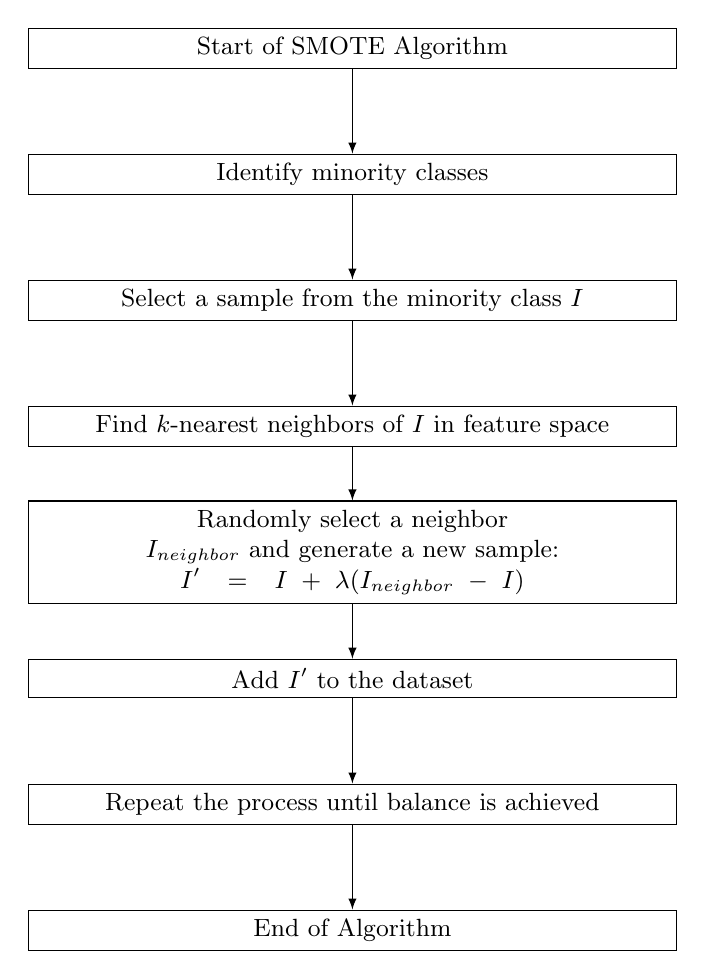
\begin{tikzpicture}[
    node distance=1.6cm,
    every node/.style={
        rectangle,
        draw,
        align=center,
        font=\small,
        text width=8cm,
    },
    >=latex, auto, font=\small
]

\node (start) {Start of SMOTE Algorithm};
\node (identify) [below of=start] {Identify minority classes};
\node (select) [below of=identify] {Select a sample from the minority class \( I \)};
\node (knn) [below of=select] {Find \( k \)-nearest neighbors of \( I \) in feature space};
\node (create) [below of=knn] {Randomly select a neighbor \( I_{\text{neighbor}} \) and generate a new sample: \\ \( I' = I + \lambda (I_{\text{neighbor}} - I) \)};
\node (add) [below of=create] {Add \( I' \) to the dataset};
\node (iterate) [below of=add] {Repeat the process until balance is achieved};
\node (end) [below of=iterate] {End of Algorithm};

\draw[->] (start) -- (identify);
\draw[->] (identify) -- (select);
\draw[->] (select) -- (knn);
\draw[->] (knn) -- (create);
\draw[->] (create) -- (add);
\draw[->] (add) -- (iterate);
\draw[->] (iterate) -- (end);

\end{tikzpicture}
\caption{فلوچارت الگوریتم SMOTE}
\label{fig:smote-flowchart}
\end{figure}
\subsection{فلوچارت وزن‌دهی در تابع هزینه}
این فلوچارت فرآیند اختصاص وزن به کلاس‌ها در تابع هزینه را برای کاهش تأثیر داده‌های نامتعادل تشریح می‌کند (شکل~\ref{fig:weighting-flowchart}).

\begin{figure}[ht]
\centering
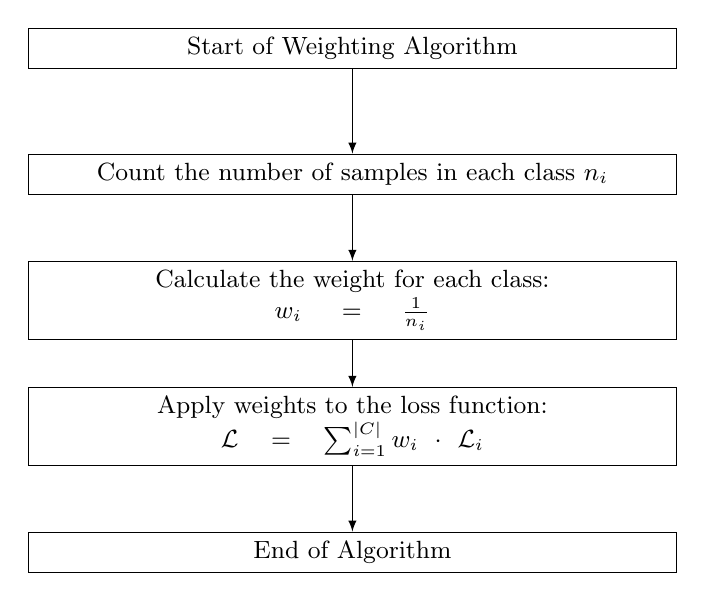
\begin{tikzpicture}[
    node distance=1.6cm,
    every node/.style={
        rectangle,
        draw,
        align=center,
        font=\small,
        text width=8cm,
    },
    >=latex, auto, font=\small
]

\node (start) {Start of Weighting Algorithm};
\node (count) [below of=start] {Count the number of samples in each class \( n_i \)};
\node (weight_calc) [below of=count] {Calculate the weight for each class: \\ \( w_i = \frac{1}{n_i} \)};
\node (apply_loss) [below of=weight_calc] {Apply weights to the loss function: \\ \( \mathcal{L} = \sum_{i=1}^{|C|} w_i \cdot \mathcal{L}_i \)};
\node (end) [below of=apply_loss] {End of Algorithm};

\draw[->] (start) -- (count);
\draw[->] (count) -- (weight_calc);
\draw[->] (weight_calc) -- (apply_loss);
\draw[->] (apply_loss) -- (end);

\end{tikzpicture}
\caption{فلوچارت وزن‌دهی در تابع هزینه}

%------------------------------------------------------------------


\label{fig:weighting-flowchart}
\end{figure}
%------------------------------------------------------------------
%   NEW SECTION (MORE PROFESSIONAL, WITH \lr{} USAGE)
%------------------------------------------------------------------

\section{مروری بر روش های افزایش داده}
در این بخش، چهار روش اصلی برای غنی‌سازی و متوازن‌سازی داده‌ها معرفی می‌گردد که در پروژهٔ حاضر تأثیر قابل‌توجهی داشته‌اند. هر یک از این روش‌ها، به‌صورت مستقل یا در ترکیب با یکدیگر، می‌تواند در سامانه‌های مختلف (از محیط‌های آزمایشگاهی تا سیستم‌های تولیدی در مقیاس وسیع) مورد استفاده قرار گیرد.

\begin{itemize}
    \item \textbf{چرخش تصادفی \lr{(Random Rotation)}:}
    با اعمال زوایای مختلف بر تصاویر ورودی، سامانه می‌تواند الگوهای چرخیدهٔ تابلوها را نیز تشخیص دهد. این روش، به‌ویژه در مواردی که تصاویر به شکل اتفاقی یا از دوربین‌هایی با زوایای غیرثابت ثبت می‌شوند، اثربخشی بالایی دارد. در سطح تولید، این فرایند اغلب قبل از ذخیره‌سازی تصاویر در دیتابیس یا هنگام آماده‌سازی ک\lr{batch}ها اعمال می‌شود تا مدل در طول آموزش با تنوع زاویه مواجه گردد.

    \item \textbf{تغییر روشنایی و کنتراست \lr{(ColorJitter)}:}
    شبیه‌سازی شرایط نوری مختلف (روز، شب، هوای ابری و غیره) کمک می‌کند مدل در سناریوهای واقعی قوی‌تر عمل کند. این روش در سامانه‌های هوشمند تشخیص علائم، خصوصاً برای دوربین‌هایی با نوردهی متغیر یا در محیط‌هایی با نور ناهمگن، بسیار مفید است. در مراکز پردازشی بزرگ (نظیر \lr{HPC} یا خوشه‌های محاسباتی)، می‌توان این فرایند را به‌صورت توزیع‌شده اعمال کرد تا عملیات پیش‌پردازش سنگین پیش از مرحلهٔ آموزش انجام شود.

    \item \textbf{\lr{SMOTE} در سطح ویژگی:}
    در مواردی که برخی کلاس‌ها (مانند نوع خاصی از علائم نادر) نمونه‌های بسیار کمی داشته باشند، مدل تمایل به نادیده‌گرفتن آن‌ها پیدا می‌کند. \lr{SMOTE} با تولید نمونه‌های مصنوعی بر اساس همسایگی داده‌های واقعی در فضای ویژگی، تنوع داده را بالا می‌برد. این الگوریتم اغلب بعد از استخراج بردار ویژگی از شبکه‌های عمیق (مثلاً لایه‌های میانی \lr{CNN}) اعمال می‌گردد تا نمونه‌های کم‌تعداد تقویت شوند. در سامانه‌های مقیاس بزرگ، اجرای \lr{SMOTE} ممکن است به‌صورت دنباله‌ای (Pipeline) با سایر مراحل تحلیل داده ادغام شود.



\begin{itemize}
    \item \textbf{وزن‌دهی در تابع هزینه\LTRfootnote{Weighted Loss}:}
    اگر توزیع کلاس‌ها بسیار نامتعادل باشد، اختصاص ضرایب وزنی بالاتر به کلاس‌های کم‌نمونه در حین آموزش (مثلاً از طریق تابع آنتروپی متقاطع\LTRfootnote{CrossEntropyLoss} وزندار) مانع از غلبهٔ کلاس‌های پرتعداد می‌شود. این تکنیک در زیرساخت‌های تولیدی\LTRfootnote{Production} نیز کاربرد زیادی دارد؛ چراکه می‌توان بدون تغییر در داده‌ها، اهمیت برخی کلاس‌ها را بیشتر کرد و مدل را به سادگی بازآموزی\LTRfootnote{Retrain} نمود.
\end{itemize}

\paragraph{روش پیاده‌سازی و نکات اجرایی:}
\begin{itemize}
    \item در کتابخانهٔ پای‌تورچ\LTRfootnote{PyTorch}، می‌توان با استفاده از ترکیب تبدیل‌ها\LTRfootnote{transforms.Compose} مجموعه‌ای از تبدیلات مانند چرخش تصادفی\LTRfootnote{RandomRotation} و تغییرات رنگ\LTRfootnote{ColorJitter} را تعریف کرد. این فرایند اغلب در مرحلهٔ بارگذار داده‌ها\LTRfootnote{DataLoader} و پیش از ارسال داده به مدل انجام می‌شود تا همهٔ عملیات لازم در حین بارگیری تصاویر صورت گیرد.
    
    \item برای بهره‌گیری از تکنیک نمونه‌برداری اقلیت مصنوعی\LTRfootnote{SMOTE (Synthetic Minority Oversampling Technique)} در فضای ویژگی، ابتدا داده‌ها را از طریق شبکهٔ اولیه یا مدل از پیش‌آموزش‌دیده\LTRfootnote{Pretrained Model} عبور داده و خروجی لایه‌های میانی را استخراج می‌کنند. سپس الگوریتم SMOTE روی این بردارهای ویژگی اعمال می‌شود تا دادهٔ مصنوعی تولید گردد. در سیستم‌های بزرگ، این مرحله ممکن است در ریزخدمات\LTRfootnote{Microservices} یا ماژول‌های جداگانه انجام پذیرد.
    
    \item در مورد وزن‌دهی در تابع هزینه\LTRfootnote{Weighted Loss}، تعیین وزن هر کلاس اغلب بر اساس معکوس فراوانی آن در مجموعهٔ آموزشی انجام می‌شود. پیاده‌سازی عملی در پای‌تورچ معمولاً از طریق متد \texttt{nn.CrossEntropyLoss(weight=\dots)} صورت می‌گیرد. این روش بدون تغییر داده‌های خام، تأکید بیشتری بر کلاس‌های کم‌نمونه دارد و در مدل‌های مستقر در محیط تولید نیز به‌آسانی به‌روزرسانی می‌شود.
\end{itemize}

\noindent
ترکیب این چهار روش—چرخش تصادفی\LTRfootnote{RandomRotation}، تغییرات رنگ\LTRfootnote{ColorJitter}، تکنیک نمونه‌برداری \texttt{SMOTE} و وزن‌دهی در تابع هزینه\LTRfootnote{Weighted Loss}—به افزایش تنوع داده و رفع مشکل عدم‌تعادل کمک می‌کند. نتیجهٔ این امر، دستیابی به مدلی است که در محیط‌های واقعی و در مواجهه با موقعیت‌های متنوع، دقت و پایداری بیشتری از خود نشان می‌دهد.


\section{معیارهای ارزیابی و مقایسه روش‌ها}

پس از اینکه داده‌هایمان را روی مدل آموزش دادیم، نیاز به ارزش‌یابی مدل و روش‌های استفاده‌شده داریم. همچنین برای مقایسه روش‌های مختلف، معیارهای ارزیابی اهمیت بسیاری دارند. در این بخش، چند مورد از معیارهای ارزیابی مدل‌ها همراه با معادل انگلیسی آن‌ها و فرمول‌ها معرفی و توضیح داده می‌شود.

دقت کلی\footnote{\lr{Accuracy}} یکی از ابتدایی‌ترین معیارها برای سنجش عملکرد مدل است که نسبت پیش‌بینی‌های صحیح مدل را صرف نظر از نوع کلاس نشان می‌دهد. این معیار برای مجموعه داده‌هایی که تعداد نمونه‌های هر کلاس تقریباً برابر است و نسبت عدم‌توازن\footnote{\lr{Imbalance Ratio}} نزدیک به \lr{1} است، یک شاخص مناسب محسوب می‌شود. با این حال، برای داده‌هایی که کلاس‌های نادر دارند، دقت کلی ممکن است تصویر اشتباهی از عملکرد مدل ارائه دهد. فرمول محاسبه نسبت عدم‌توازن و دقت کلی به شکل زیر است:

\begin{equation}
\text{\lr{Imbalance Ratio}} = \frac{\text{تعداد نمونه‌های بزرگ‌ترین کلاس}}{\text{تعداد نمونه‌های کوچک‌ترین کلاس}}
\end{equation}

\begin{equation}
\text{\lr{Accuracy}} = \frac{TP + TN}{TP + TN + FP + FN}
\end{equation}

دقت پیش‌بینی مثبت‌ها\footnote{\lr{Precision}} شاخص دیگری است که تمرکز آن بر درصد نمونه‌هایی است که به درستی به‌عنوان مثبت پیش‌بینی شده‌اند. این معیار زمانی اهمیت پیدا می‌کند که پیش‌بینی اشتباه یک کلاس مثبت هزینه بالایی داشته باشد. به عنوان مثال، در شناسایی علائم راهنمایی و رانندگی، اشتباه در پیش‌بینی علائم ایست یا سرعت می‌تواند منجر به حوادث خطرناک یا جریمه راننده شود. فرمول محاسبه این معیار به صورت زیر است:

\begin{equation}
\text{\lr{Precision}} = \frac{TP}{TP + FP}
\end{equation}

نرخ بازخوانی\footnote{\lr{Recall}} یا حساسیت، شاخصی است که توانایی مدل در شناسایی تمامی نمونه‌های مثبت واقعی را اندازه‌گیری می‌کند. این معیار در شناسایی علائم ترافیکی با اهمیت بالا، مانند علائم هشداردهنده یا محدودیت سرعت، بسیار کاربرد دارد. از دست دادن شناسایی این علائم، که به خطای منفی کاذب منجر می‌شود، می‌تواند اثرات جدی داشته باشد. فرمول محاسبه نرخ بازخوانی به شرح زیر است:

\begin{equation}
\text{\lr{Recall}} = \frac{TP}{TP + FN}
\end{equation}

امتیاز \lr{F1}\footnote{\lr{F1 Score}} به عنوان میانگین هارمونیک بین \lr{Precision} و \lr{Recall} تعریف می‌شود. این معیار به‌ویژه زمانی اهمیت پیدا می‌کند که داده‌ها نامتوازن باشند و نیاز به ارزیابی عملکرد مدل در شناسایی هر دو نوع خطای مثبت کاذب و منفی کاذب وجود داشته باشد. فرمول امتیاز \lr{F1} به شکل زیر است:

\begin{equation}
\text{\lr{F1}} = \lr{2} \times \frac{\text{\lr{Precision}} \cdot \text{\lr{Recall}}}{\text{\lr{Precision}} + \text{\lr{Recall}}}
\end{equation}

نرخ مثبت کاذب\footnote{\lr{False Positive Rate}} نشان می‌دهد که مدل چه تعداد از نمونه‌های منفی واقعی را به‌اشتباه به‌عنوان مثبت پیش‌بینی کرده است. از سوی دیگر، نرخ منفی کاذب\footnote{\lr{False Negative Rate}} مشخص می‌کند که مدل چه تعداد از نمونه‌های مثبت واقعی را نتوانسته شناسایی کند. فرمول این معیارها به صورت زیر تعریف می‌شوند:

\begin{equation}
\text{\lr{FPR}} = \frac{FP}{FP + TN}
\end{equation}

\begin{equation}
\text{\lr{FNR}} = \frac{FN}{FN + TP}
\end{equation}

منحنی \lr{ROC}\footnote{\lr{Receiver Operating Characteristic}} ارتباط بین \lr{Recall} و نرخ مثبت کاذب\footnote{\lr{False Positive Rate (FPR)}} را نمایش می‌دهد. مساحت زیر این منحنی\footnote{\lr{Area Under Curve (AUC)}} توانایی کلی مدل در تفکیک بین کلاس‌های مختلف را نشان می‌دهد. این معیار برای مدل‌هایی که احتمالات پیش‌بینی می‌کنند، مانند شبکه‌های عمیق، کاربرد ویژه‌ای دارد. فرمول محاسبه مساحت زیر منحنی \lr{ROC} به شرح زیر است:

\begin{equation}
\text{\lr{AUC}} = \int_{0}^{1} \text{\lr{ROC}}(x) dx
\end{equation}

در کنار این معیارها، ماتریس سردرگمی\footnote{\lr{Confusion Matrix}} ابزاری گرافیکی است که عملکرد مدل را با تقسیم پیش‌بینی‌ها به چهار دسته نشان می‌دهد:
\begin{figure}[h!]
\centering

\includegraphics[width=0.5\textwidth]{cof_matrix}
\caption{ماتریس سردرگمی برای مدل مورد بررسی}
\label{fig:confusion_matrix}
\end{figure}





این ماتریس برای تحلیل نقاط ضعف مدل و شناسایی کلاس‌هایی که بیشتر با یکدیگر اشتباه گرفته می‌شوند، بسیار مفید است.

در مقایسه مدل‌ها، معمولاً از ترکیبی از این معیارها استفاده می‌شود تا نقاط قوت و ضعف هر مدل به طور کامل مشخص گردد. به عنوان مثال:
\begin{itemize}
    \item مدل‌های سنتی مبتنی بر ویژگی‌های رنگ و شکل ممکن است در معیارهایی نظیر \lr{Specificity} عملکرد بهتری داشته باشند.
    \item مدل‌های یادگیری عمیق مانند شبکه‌های \lr{CNN}\footnote{\lr{Convolutional Neural Networks}} یا مدل‌های مبتنی بر \lr{Transformer}\footnote{\lr{Transformer-based Models}} معمولاً در معیارهایی نظیر \lr{AUC-ROC} و \lr{Recall} برجسته‌تر هستند.
\end{itemize}
section{مدل‌ها}
\subsection{\lr{MobileNetV2}}
\label{sec:MobileNetV2}

مدل \lr{MobileNetV2} یک شبکه عصبی کانولوشنی است که برای پردازش تصاویر طراحی شده است و به‌ویژه برای دستگاه‌های موبایل و سیستم‌های با منابع محدود بهینه‌سازی شده است. این مدل از تکنیک‌های نوینی مانند Inverted Residuals و Linear Bottlenecks بهره می‌برد که موجب کاهش پیچیدگی محاسباتی و افزایش کارایی در مقایسه با سایر مدل‌های مشابه می‌شود. از دیگر ویژگی‌های مهم این مدل، ساختار لایه‌های کانولوشنی به‌صورت Depthwise Separable Convolution است که در آن عملیات کانولوشن به دو بخش تقسیم می‌شود: کانولوشن عمقی و کانولوشن نقطه‌ای. این رویکرد باعث می‌شود که تعداد پارامترها به‌شدت کاهش یابد و در نتیجه، سرعت پردازش مدل افزایش یابد.

در مدل \lr{MobileNetV2}، به‌جای استفاده از کانولوشن‌های سنتی، از یک ساختار جدید به نام Inverted Residuals استفاده می‌شود که در آن ابتدا یک لایه‌ی عریض با تعداد فیلتر بیشتر به‌وجود می‌آید و سپس با استفاده از Linear Bottleneck به‌طور مؤثری ابعاد ویژگی کاهش می‌یابد. این رویکرد باعث می‌شود که مدل بتواند ویژگی‌های پیچیده‌تری را در لایه‌های اولیه استخراج کند و در عین حال از لحاظ محاسباتی بهینه باشد.

این مدل، برای بسیاری از کاربردهای بینایی کامپیوتری مانند شناسایی اشیاء، طبقه‌بندی تصاویر و تشخیص ویژگی‌ها در موبایل‌ها و دستگاه‌های کم‌قدرت به‌طور مؤثری مورد استفاده قرار می‌گیرد.

\begin{figure}[h!] \centering 
\includegraphics[width=0.8\textwidth]{Mobile_Fig_01} \caption{معماری شبکه عصبی \lr{MobileNetV2}} \label{fig:Mobile_Fig_01} \end{figure}

\subsection{\lr{EfficientNet}}
\label{sec:EfficientNet}

مدل \lr{EfficientNet} یکی از مدل‌های جدید و پیشرفته شبکه‌های عصبی است که توسط تیم Google AI در سال 2019 معرفی شد. این مدل به‌طور قابل توجهی نسبت به مدل‌های مشابه مانند \lr{ResNet} و \lr{MobileNet} بهینه‌تر است و برای بهبود کارایی شبکه‌های عصبی از یک رویکرد به نام Compound Scaling استفاده می‌کند. به‌عبارت دیگر، در این مدل علاوه بر افزایش عمق شبکه، مقیاس‌های دیگر مانند عرض شبکه و وضوح تصویر نیز به‌طور هم‌زمان افزایش می‌یابد تا کارایی بالاتری برای پردازش تصاویر به‌دست آید.

یکی از ویژگی‌های برجسته این مدل، کاهش Overhead در محاسبات و حافظه است. به‌طور معمول، افزایش عمق شبکه موجب افزایش میزان محاسبات و حافظه مصرفی می‌شود، اما با استفاده از رویکرد Compound Scaling در \lr{EfficientNet}، به‌طور هم‌زمان ابعاد دیگر (عرض و وضوح) به‌صورت هوشمندانه‌ای افزایش می‌یابد تا مدل بهینه‌تر و با دقت بالاتری عمل کند.

این مدل نه‌تنها تعداد پارامترها را کاهش داده، بلکه دقت بیشتری در انجام وظایف بینایی کامپیوتری ارائه می‌دهد. \lr{EfficientNet} به‌ویژه برای کار در محیط‌های با محدودیت منابع بسیار مناسب است و در بسیاری از کاربردهای پیشرفته، مانند تشخیص تصاویر در پزشکی و شناسایی اشیاء، موفقیت‌های بزرگی داشته است.

\begin{figure}[h!] \centering 
\includegraphics[width=0.8\textwidth]{EfficientNet_Fig_01} \caption{معماری \lr{EfficientNet}} \label{fig:EfficientNet_Fig_01} \end{figure}

\subsection{\lr{ResNet}} 
\label{sec:ResNet}

مدل \lr{ResNet} (\lr{Residual Networks}) یکی از موفق‌ترین و پرکاربردترین مدل‌های شبکه عصبی است که در سال 2015 توسط \lr{Kaiming He} و همکارانش معرفی شد. این مدل به‌ویژه برای شبکه‌های عمیق طراحی شده و از \lr{Residual Learning} برای حل مشکل ناپدید شدن گرادیان در شبکه‌های عصبی عمیق بهره می‌برد. یکی از مشکلات اصلی در شبکه‌های عصبی عمیق، \lr{Vanishing Gradient Problem} است که باعث می‌شود آموزش شبکه‌های با عمق زیاد بسیار دشوار و زمان‌بر شود. برای مقابله با این مشکل، \lr{ResNet} از \lr{Skip Connections} یا \lr{Residual Blocks} استفاده می‌کند که به شبکه این امکان را می‌دهد تا مسیرهای کوتاه‌تری برای جریان گرادیان‌ها داشته باشد، در نتیجه، شبکه می‌تواند به‌طور مؤثری و بدون مشکل ناپدید شدن گرادیان، آموزش ببیند.

در مدل \lr{ResNet}، از یک یا چند بلوک \lr{Residual} استفاده می‌شود که در آن ورودی هر لایه به خروجی لایه‌ی بعدی اضافه می‌شود. این روش باعث می‌شود که شبکه به راحتی به عمق‌های بیشتر گسترش یابد بدون آنکه مشکلات یادگیری ایجاد شود. این مدل در سال‌های اخیر در بسیاری از رقابت‌ها و کاربردهای بینایی کامپیوتری به موفقیت‌های زیادی دست یافته است.

\begin{figure}[h!] \centering 
\includegraphics[width=1.0\textwidth]{ResNet_Fig_01} \caption{معماری \lr{ResNet}} \label{fig:ResNet_Fig_01} \end{figure}

\subsection{ساختار معماری و اجزای اصلی}
\label{subsec:Mobile_Fig_01}

در یک نگاه کلی، ساختار مدل‌های ذکرشده را می‌توان به دو بخش اصلی تقسیم کرد:

\begin{enumerate}
    \item \textbf{بخش کانولوشنی (\lr{Convolutional Part}):}
    شبکه‌های کانولوشنی با لایه‌های مختلف و فیلترهایی در ابعاد گوناگون، به‌دنبال شناسایی ویژگی‌های موضعی در سطح فرکانس-زمان (یا هر فضای ویژگی دیگر) هستند. خروجی این بخش، معمولاً یک نگاشت ویژگی \LTRfootnote{\lr{Feature Map}} چندکاناله است که در هر مقطع زمانی، اطلاعات فشرده‌ای از الگوهای محلی \LTRfootnote{\lr{Local Patterns}} را ذخیره می‌کند.
    \item \textbf{بخش تمام‌اتصال (\lr{Fully Connected Part}):}
    پس از استخراج ویژگی‌های موضعی، معمولاً شبکه‌های عصبی به لایه‌های تمام‌اتصال یا \lr{fully connected} متصل می‌شوند تا ویژگی‌های استخراج‌شده را برای تصمیم‌گیری‌های نهایی پردازش کنند. در مدل‌هایی مانند \lr{ResNet} و \lr{MobileNetV2}، این لایه‌ها اغلب با استفاده از کلاس‌های خروجی و توابع فعال‌سازی مانند \lr{Softmax} برای طبقه‌بندی تصاویر استفاده می‌شوند.
\end{enumerate}


\subsection{مکانیزم آموزش و روش‌های ارزیابی}
\label{subsec:CNN-RNN-Training-Eval}

برای \textbf{آموزش} این مدل‌ها، ابتدا یک تابع هزینه مناسب تعریف می‌شود و سپس وزن‌های شبکه با استفاده از روش‌های بهینه‌سازی گرادیان‌محور نظیر \lr{Adam}\LTRfootnote{Adaptive Moment Estimation} یا \lr{SGD}\LTRfootnote{Stochastic Gradient Descent} به‌روزرسانی می‌گردند. بسته به این‌که مسئله از نوع طبقه‌بندی یا رگرسیون باشد، می‌توان از توابعی مانند آنتروپی متقاطع (Cross-Entropy) یا \lr{MSE}\LTRfootnote{Mean Squared Error} بهره برد. همچنین، برای جلوگیری از بیش‌برازش، روش‌هایی نظیر دراپ‌آوت \LTRfootnote{Dropout}، توقف زودهنگام \LTRfootnote{Early Stopping} و تنبیه وزن \LTRfootnote{Weight Decay} متداول هستند.

در مرحلۀ \textbf{ارزیابی} مدل، معیارهای موفقیت به نوع مسئله وابسته است: \begin{itemize} \item در سناریوهای طبقه‌بندی (مانند تشخیص اشیاء)، معیارهایی نظیر دقت \LTRfootnote{Accuracy}، امتیاز \lr{F1}\LTRfootnote{F1-Score}، \lr{Precision}\LTRfootnote{Precision} و \lr{Recall}\LTRfootnote{Recall} کاربرد دارند. \item در وظایف پیش‌بینی یا بازتولید سیگنال، معیارهایی نظیر \lr{RMSE}\LTRfootnote{Root Mean Squared Error}، \lr{MAE}\LTRfootnote{Mean Absolute Error} یا ضریب تعیین \lr{R^2}\LTRfootnote{Coefficient of Determination} به‌کار گرفته می‌شوند. \end{itemize}

ارزیابی مدل با این شاخص‌ها، میزان بهبود مدل ترکیبی را در مقایسه با روش‌های دیگر ـ یا در مقایسه با بهره‌گیری جداگانه از \lr{CNN} و \lr{RNN} ـ روشن‌تر می‌کند.